%! Author = Administrator
%! Date = 2021/7/2

\chapter{需求分析}
本章将结合需要实现的基本功能和优化目标,在原系统的基础上,修改原有的系统架构以期改进执行的效率。通过对应用服务编排系统的国内外公司相
似产品进行调研,以及公司现有的公有云体系设计相结合,针对系统的需求分析进行阐述。

\section{产品分析}
ASW是一个可视化的服务编排云服务,用于直观地构建应用工作流,简化开发,进行任务协调、状态管理、错误处理等繁琐工作。
系统现有架构如下:

\begin{figure}[h]
    \centering
    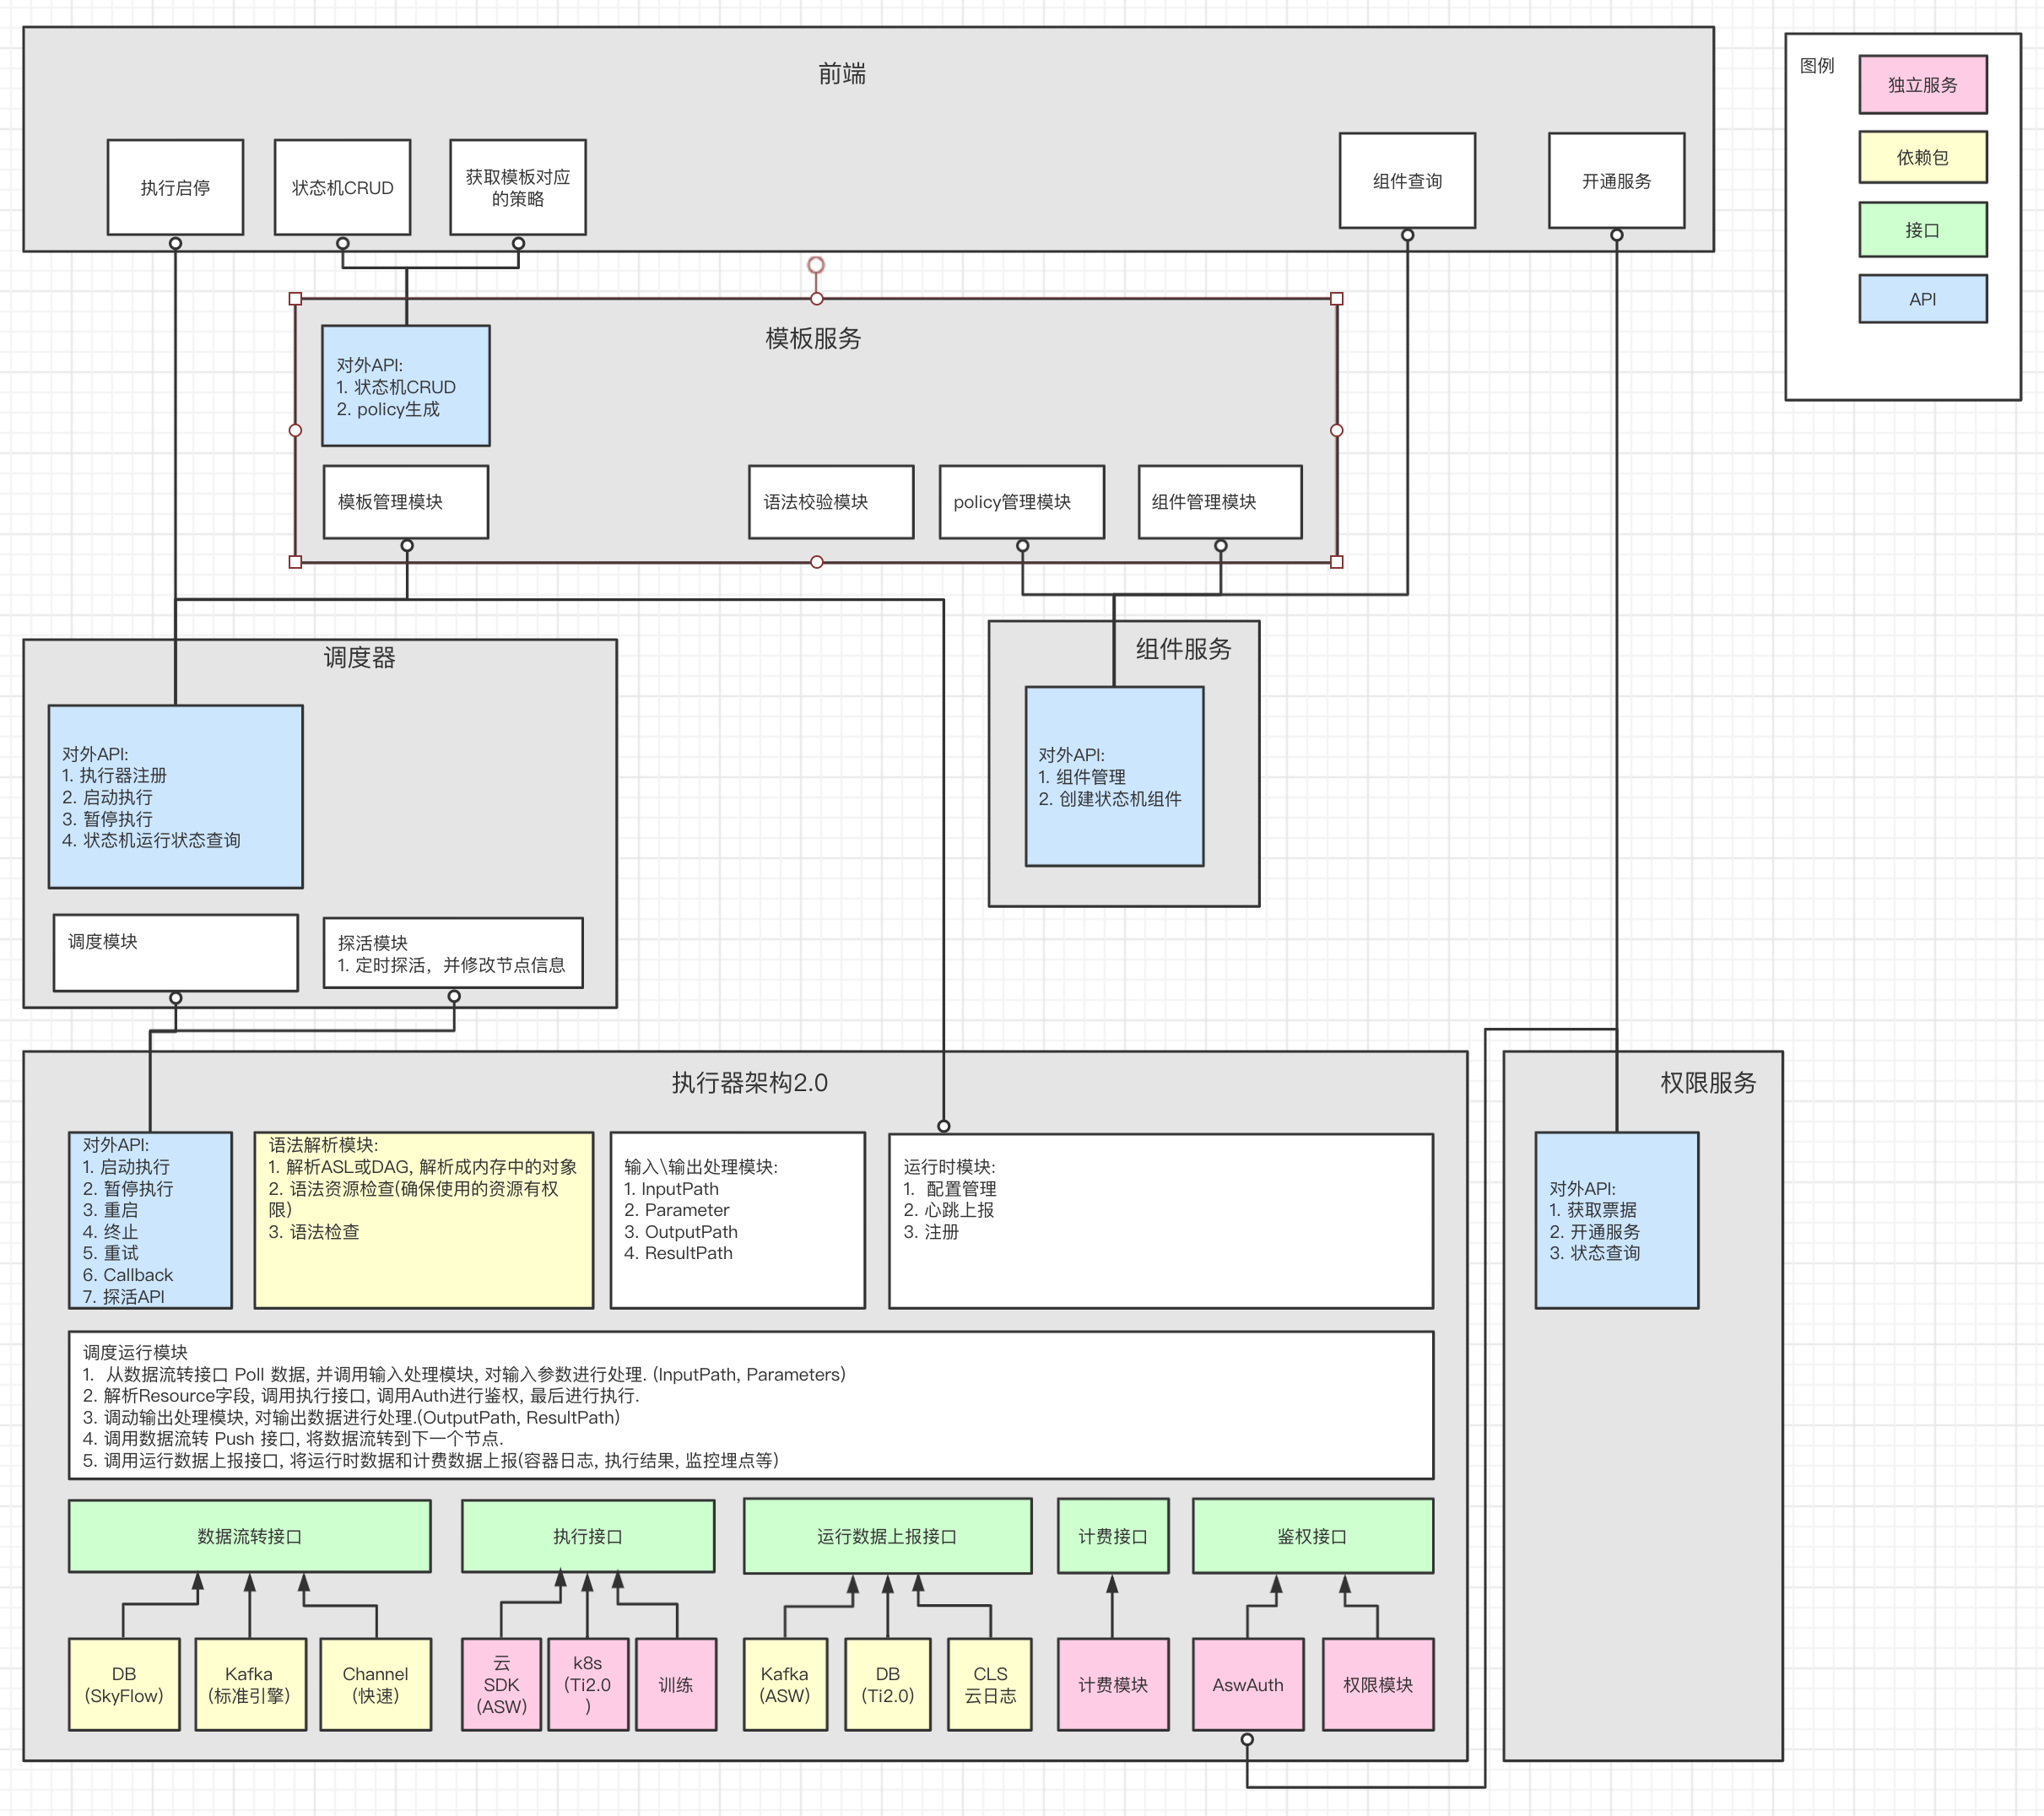
\includegraphics[width=1.2\textwidth]{3-1.jpg}
    \caption{ASW系统架构设计图}
    \label{fig:xtjg}
\end{figure}

根据图1.1,可见执行器是整个系统的核心模块,其中涉及模块多,实现逻辑复杂,大量的优化措施都是针对执行器的,而执行器的执行效率就是一个
很重要的指标,它反映了整个服务的质量。可以看到,在执行器的调度运行模块当中,这部分的设计借鉴了亚马逊Step Functions的设计思路,通过
构建DAG,并对其进行解析,部署到容器顺序执行[1]。

本产品旨在设计一种能够将各种云服务功能模块组合到功能丰富的应用程序中的工作流。工作流由一系列步骤组成,其中一个步骤的输出将作为下一个
步骤的输入。

将工作流转换为易于理解、易于解释和易于更改的状态机图,可以监控执行的每个步骤,这意味着能够快速发现和修复问题。通过自动触发和跟踪每个
步骤,并在出现错误时重试,可以保证应用程序会按顺序正常执行。无需进行繁琐的状态机编程,而是通过JSON结构化语言来进行配置工作流。

\begin{figure}[H]
    \centering
    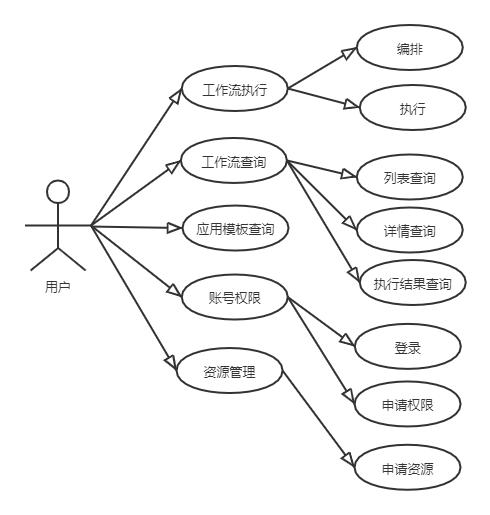
\includegraphics[width=0.9\textwidth]{user-1.png}
    \caption{用户用例图}
    \label{fig:yhyl}
\end{figure}

如图所示,用户主要的诉求是工作流的编排、查询和执行。在对这三种复合型任务进行需求拆解分析时,必须要进行单独拆分,将工作流编排和执行分开,前者主要对应
的是模板服务,后者主要是调度器服务和执行器服务。将权限管理单独组成一个模块,管理用户执行权限、资源权限等。这样,系统的大致划分就完成了。
进一步地,需要对各个功能点进行更全面的考虑。以下,从功能性需求、非功能性需求两个大类进行分类讨论。

\begin{figure}[H]
    \centering
    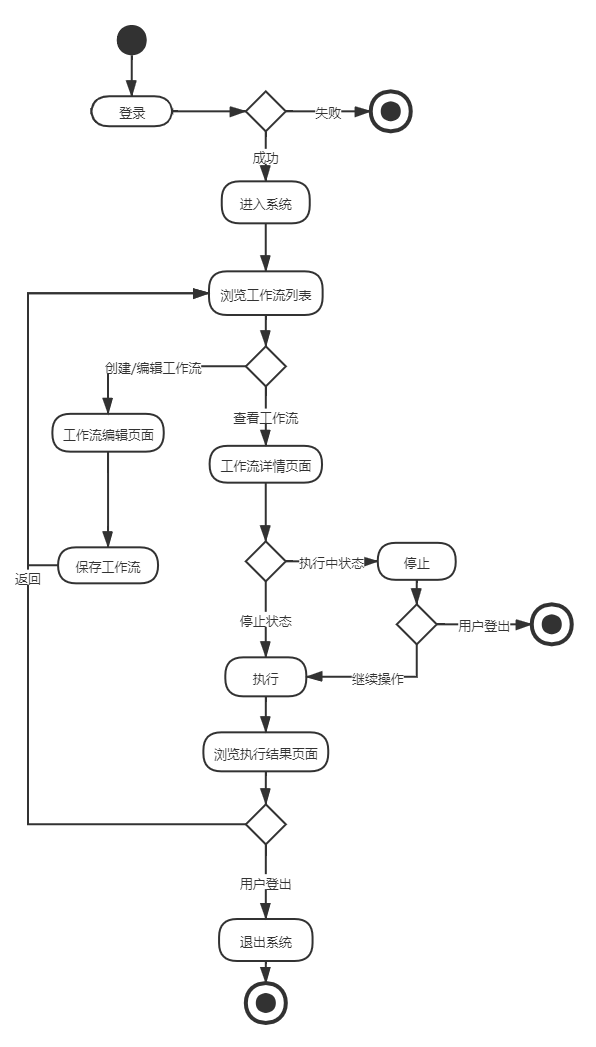
\includegraphics[width=1.0\textwidth]{activity-user.png}
    \caption{用户活动图}
    \label{fig:yhhd}
    \note{}
\end{figure}

如上图所示,用户从登录系统到退出系统,大致符合这样一套流程,提供的核心服务是工作流的各种操作,用户可能需要申请权限以登录到本系统。系统将会为用户
新增一条用户数据,以便以后追踪该用户创建、执行的工作流,以及配置信息。

在使用时,用户可以根据系统界面的指导,完成对系统的初步熟悉。第一次时,可能会经历如下的流程:浏览工作流列表,根据应用模板创建工作流,执行工作流,
查询工作流执行结果。这是一套最小流程,即在图中的最短路径,可以体验一次云服务应用编排带来的实用性和便捷性。

同时,系统还应提供一些高级功能,比如编辑自定义工作流,用户可以定制除了预设模板以外的符合自己需求的工作流,比如带有并行执行,循环执行任务的工作流;
在创建了较多工作流时,可能会使用到工作流排序、模糊查询等功能,并且,系统支持查询7天以内所有执行过的工作流日志,都会保存在系统之中,方便用户自行
排查错误。



\section{功能性需求}
基于对用户需求的提炼分析,针对功能性方面的需求,总结出如下几个部分。

\subsection{工作流编排}
工作流编排是指用户通过可视化的形式,构建自己想要的工作流。可选地,使用TCSL,也可以构建一个工作流。可视化编排的输出,也是TCSL定义,
编排的工作,就是理解用户需求,将用户的需求转化为系统可以理解的语言结构。这里,TCSL即是一个自然语言和机器语言的中间语言,完成了用户与
机器沟通的桥梁作用。

编排功能的引入是为了让用户使用的门槛降至最低,可以将用户的注意力放在设计自己的工作流上,而不是如何使用我们的系统,徒增使用成本。
设计初衷是将复杂的流程简单化,提供用户友好型界面,使专业背景不同的用户都可以流畅地使用。

编排界面应包括组件管理界面,提供可供编排的组件列表,比如并行节点、条件选择节点、循环迭代节点等常用流程管理的节点,以及公有云服务算法节点。其中,
流程管理节点指的是如同编程时使用的IF、For语句一样,对程序进行条件分支转移,这里也一样,通过这些节点来根据一定的条件,进行后续不同节点
的选择执行。而公有云服务算法节点,包含所有公有云的可用算法,比如视频转码、语音合成、翻译、自定义云函数等,都能够以一个节点的形式,作为
工作流的一部分,一个执行环节。 进一步地,云函数是一个Serverless形式的公有云自定义函数服务,可以执行各种后段语言编写的函数。这种服务的
优点是以Serverless的模式运行,不需要维护自己的服务器\cite{Jeffery_2021}。缺点也是显而易见的,由于其没有固定的服务器,因此,如何运行通常面临着不确定性,无法统一调度,
而本系统则正好解决了云函数没法统一编排调度的一个缺陷,也使得云函数更具有实用价值。这即是一个云服务之间互相协同工作,一加一大于二的例子。
工作流编排可以使云服务锦上添花。

\subsection{工作流管理}
工作流管理包括工作流的创建、修改、删除、执行等操作。

工作流执行是系统的主要功能。实现该功能,需要本系统所有模块的共同协作,工作流的执行会使得数据流转到调度器、执行器最终返回给用户,是一个
流程链路很长的一类功能。

用户根据业务场景,使用自己构建工作流,需要提供简易、可用的执行功能。用户应可对每次工作流的执行提供输入,以JSON的形式给出,
用户可以方便地进行保存以及复用。在执行完毕后,用户应可以查看本次执行结果的成功与否。



\subsection{查询工作流详情}

用户希望可以直观明确地查询到其提交的工作流任务执行的情况,包括工作流列表、工作流执行记录。
对每个工作流,都提供相应的界面可以直观地

工作流详情页面需求内容:
DAG节点执行情况:本工作流所有节点使用ECharts展示,完成情况也应实时进行刷新反馈给用户。

工作流执行记录:包括该次执行时提供的输入和执行结果。

\subsection{工作流应用模板部署}

用户使用工作流门槛较高,希望有一种方式可以快速构建一个具体场景的工作流。

用户自定义的工作流为普通工作流,储存在各个用户名下。而这种工作流称为应用模板工作流,预设计好的一种方便用户快速构建常见业务场景的一种
工作流。如视频切片转码、医疗单项报告整合分析等,都可以作为场景向用户进行提供。由于该功能涉及资源较多,因此也需要单独抽取出来,与普通
的用户自定义工作流执行作出区分,增加相应的资源申请步骤。


核心问题
\begin{itemize}
    \item 由于创建模板,往往需要操作用户名下的很多种类的资源,因此需要在构建工作流时,将依赖的资源一起创建
    \item 可方便的横向扩展,今后由技术运营进行相关的配置和开发,就能添加更多的模板
    \item 复用现有能力:使用应用模板创建出的工作流,能按照现有工作流的逻辑进行查看、运行、更新、删除
\end{itemize}

\subsection{工作流应用模板查询}

系统提供一些常见业务场景下编排好的工作流,用户应可用实时查看到这些可用的工作流,并以此为基础来客制化他们需要的服务需求。

要查询这些模板,也同样需要和普通工作流执行作区分,将查询封装成单独的接口,因为其需要提供很多额外的信息,才能帮助用户创建好所需的所有
资源,使得其工作流可以得到正常的执行。

\subsection{权限管理}
由于系统涉及多方资源调用,用户敏感信息等,需要一个统一的权限管理方式对整个系统进行用户权限的分级和验证。以AOP编程思想\[1\],增设一个额外的微服务模块作为鉴权模块,
将权限检查和业务逻辑解耦合,方便日后对其进行改动时,不用改动业务代码,只需要对该微服务模块进行改动和替换即可。


用户服务包含用户注册、用户状态查询、用户注销等功能,对每一个需要使用本系统的用户,都记录在数据库中,保存用户的状态。

由于本系统需要调用外部服务,因此增设日志管理类ActionLog,用以记录每次鉴权和用户注册、用户注销的记录,便于数据分析与问题的排查。


\section{非功能性需求}

\subsection{预测执行}

主要职责是维护容器节点的状态与任务执行。前者借助Kubernetes实现;后者是本系统核心功能部分,执行DAG所有节点,进行节点间数据流转,输出
执行结果。该部分业务职责单一,但并发量需求大,所以需要尽可能减少耗时的操作,影响效率的操作应该放至模板模块中进行。




此外,根据实际情况,如图4-x,可以发现大多数节点的输出都是布尔值,整数或短字符串,少数情况下是URL、复杂字符串。可以根据这一特点,将需
要前置节点输出才能执行的节点进行统计预测,根据预测的结果,提前执行所有的节点,如果预测的输入和前置节点实际执行的结果一样,就可以做到时间
复杂度为O(max(Time(Node\_i))),远远比普通执行器的O(Sum(Time(Node\_i)))要快。


下表4-x,是该工作流执行的过程:

第一轮执行:
\begin{table}[H]
    \centering
    \caption{预测执行过程第一轮}
    \label{tab:predict_process_1}
    \begin{tabular}{llllll}
        \toprule
        节点 &实际输入 &预测输入 &正确输出 &预测输出 &节点逻辑伪代码\\
        \midrule
        1 &null    &null   &1       &1       &return 1 \\
        2 &1       &1      &2       &2       &return preInput == 1 ? preInput + 1 : -1 \\
        3 &2       &2      &4       &4       &return preInput == 2 ? preInput * 2 : -1 \\
        4 &4       &3      &-1      &6       &return preInput == 3 ? preInput * 2 : -1 \\
        \bottomrule
    \end{tabular}
\end{table}
由于最后一个节点的实际输入≠预测输入,因此不能使用预测执行器给出的结果:6,但前三个节点的预测输入都正确,因此仅将最后一个节点退化为使
用实际输入执行重新计算,如下表4-x第二轮执行:

\begin{table}[H]
    \centering
    \caption{预测执行过程第二轮}
    \label{tab:predict_process_2}
    \begin{tabular}{llllll}
        \toprule
        节点 &实际输入 &预测输入 &正确输出 &预测输出 &节点逻辑伪代码\\
        \midrule
        1 &4       &null      &-1      &null       &return preInput == 3 ? preInput * 2 : -1
    \end{tabular}
\end{table}

得到正确的结果:-1,此时,已执行到最后一个节点,结束执行。假设4个任务节点时间开销为1个时间单位, 空间开销为1个空间单位,则预测执行器
和普通执行器的总体开销对比如下表4-x:

\begin{table}[H]
    \centering
    \caption{开销对比(时间开销 / 空间开销)}
    \label{tab:cost}
    \begin{tabular}{llllll}
        \toprule
        普通执行器 & 预测执行器 & 提升比例 \\
        \midrule
        4 / 1   &2 / 4   &200\% / -400\% \\
        \bottomrule
    \end{tabular}
\end{table}

可以看出,即使代价是多使用了4倍的容器数量,但得到的时间开销200\%提升在工程实践上意义是不言而喻的,因为容器可以通过增加CPU核心数,机
房机器数进行横向扩容,数量仅受限于预算,而不在技术层面。在理论上,预测结果正确的一次执行可以达到无论节点数量,时间开销都低至O(1),
最坏情况退化到O(n)。

%\subsection{动态负载探活}
%启动执行 负载均衡 查询t\_processor表 执行器负载上报周期, 如果过短(可能是1秒).
%
%在计算负载时, 会错误的认为某个执行器还比较闲, 因此会高优先级派发任务.


%\subsection{内存管理优化}
%
%内存泄漏问题会在系统业务量不断提升,系统复杂度日益增加的情况下,是一个需要高度重视加以解决的问题,否则将影响整个系统的日常运行。
%
%执行器内存泄漏,如下图。
%
%\begin{figure}[H]
%    \centering
%    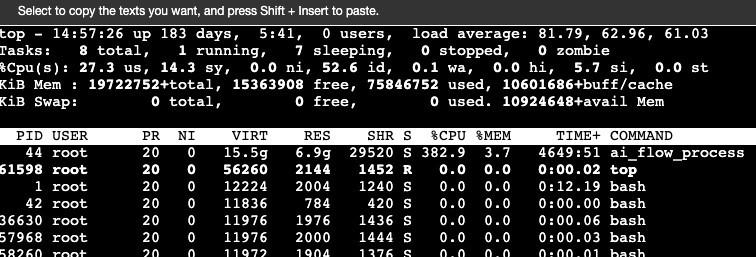
\includegraphics[width=1.0\textwidth]{3-4.jpg}
%    \caption{内存使用状态}
%    \label{fig:ncsyzt}
%\end{figure}
%
%隔一段时间就会发生OOM(Out Of Memory)错误。
%
%对执行任务时的整个系统业务流程进行纵向抽象后,可以分为模板任务引擎和执行服务引擎。引擎接受的任务均可以抽象为不同的执行步骤,每个步骤是一个节
%点,这个节点如果不是End节点,则会继续向服务引擎下发任务,对这个节点的任务做进一步的拆解。所以这两个服务接受了接入层的请求之后,所做的工作主要是以下内容:
%
%构造出一个DAG节点图,并初始化各个节点
%
%下发初始节点的数据,并开始流转节点状态
%
%流转到的节点运行该节点的工作,例如请求某一个外部服务,或者继续拆解任务请求到服务引擎
%
%从上图也可以看出,大部分的耗时任务均会在服务引擎中执行。服务引擎有大量的任务需要请求繁重的算法任务,比如视频解码时使用的抽帧解码算法,
%所以当视频文件很大、时间很长的情况下,该引擎会接受大量的图片数据,如果不采取措施,很容易导致OOM。
%
%\subsubsection{预估内存}
%
%实际占有内存应该与任务数,节点数,节点间传输数据大小,节点传输频率相关\cite{qyjy}。
%
%我们将内存大致分为3部分:
%
%实际内存 = 初始内存 + 正在使用内存 + 来不及回收的内存
%
%其中正在使用的内存包括节点内正在使用的和部分在队列中的数据。
%
%正在使用内存=任务数 x 节点数 x 节点最大并发数 x(请求包大小x2+节点传输大小+节点额外内存)+ 队列总大小 *(节点传输大小+额外内存)
%
%来不及回收的内存主要为这段时间节点流量大小
%
%来不及回收的内存=任务数x节点数xQPSx(请求包大小x2+节点传输大小+额外内存)
%
%根据图示,我们在服务中这些关键的因素均加上了限制之后开始测试。
%为了简化测试,只运行一个任务,任务的节点数为10个,每帧大小设置为传输2M的图片,并将队列暂时关闭,主要测试并发数与QPS的影响。
%
%(以下数据均为运行一段时间后相对稳定的数据)
%
%\begin{table}[H]
%    \centering
%    \caption{内存用量测试}
%    \label{tab:member_test}
%    \begin{tabular}{llll}
%        \toprule
%        QPS\/并发数	&1	&2	&3 \\
%        \midrule
%        1	&124M	&132M &120M\\
%        1	&165M	&168M &170M\\
%        1	&320M	&420M &280M\\
%        1	&680M	&820M &920M\\
%        \bottomrule
%    \end{tabular}
%\end{table}
%
%
%根据推算的公式,我们需要对服务做如下限制:
%
%任务数限制
%\begin{itemize}
%    \item 节点最大并发数限制:并发数会影响CPU,间接影响到内存回收,所以统一全局配置
%    \item 节点间传输大小限制与请求包体限制
%    \item 节点接受数据QPS限制
%\end{itemize}

%\subsubsection{服务降级、熔断策略}
%为了应对高流量带来的挑战,无法预料用户的请求量大小会对服务产生什么样的影响,因此对后台服务和数据库进行必要的限制是必须的

\subsection{系统可靠性}
为了保证系统能够平稳可靠地在容器集群中运行,需要对系统的可靠性进行需求分析。我们从以下四个方面进行分析。
\begin{enumerate}
    \item 有效性: 系统有效性是指在系统启动的一段时间内,是否可以稳定地提供各个模块的API服务,并且返回结果正确。作为一个任务编排执
行系统,执行成功是系统价值所在,如果长期不可用,必然使接入用户的业务受到影响,可能会造成不可预计的损失,这是不可接受的。 为此,本系
统高可用架构设计下的有效性体现在节点任务执行的有效性,系统服务不可出现长时间宕机的情况。
    \item 最终一致性:对同一模板请求执行时,如果是并行节点执行,会出现顺序不一致的情况,这种情况应该被允许,用户不可查看过程节点的输入输出,
系统仅对最终结果负责,该校验器需要对每次执行的结果进行分析,对此,要将每次执行的结果进行暂存,保证每一次操作都可被追溯。相关部件有如下两个。
    \item[+] 结果缓存:隶属于执行器服务模块,需要实现预测结果的暂时存储,快速读取这些结果值。[1]
    \item[+] 预测执行:隶属于执行器服务模块,负责对结果正确性进行保证,如预测执行在某节点失败,则负责发送其余任务到普通执行器中。[1]
    \item 鲁棒性:系统的鲁棒性是评判一个系统的重要指标。由于本系统的业务流程涉及大量数据的流转和自定义输入的处理,因此,需要对输入的
有效性、合法性进行周全的检查,防止不当输入导致的系统异常和崩溃。
    \item 易恢复性:需要考虑到在一些极端条件下出现了服务不可用的情况后,系统恢复运行的速度。而制约恢复速度的两个前提条件有云平台容器
资源的申请与创建以及容器镜像的服务启动。
\end{enumerate}


%\subsection{分布式全局唯一QRN生成}
%生成执行Qrn性能过低:
%
%转化为分布式全局唯一ID问题,参考Fackbook的雪花算法实现的高效分布式全局QRN字符串生成算法。
%
%\subsection{自动化测试能力建设}
%
%\begin{itemize}
%    \item 使用go test命令进行测试
%    \item 每次测试时初始化数据库
%    \item 针对service层进行测试
%    \item 测试内容包括接口功能和代码覆盖率
%\end{itemize}

\subsection{日志巡检}

用户执行的工作流产生的记录日志在数据量庞大的时候是一个极大的负担,维护调试时如何保证高效地查询到运维人员关心的日志条目,
是一个需要考虑的问题。考虑到日志的错误情况大多数是可以复现的,因此很多的日志错误很可能是同一类型的错误,因此考虑采用日志聚类的思想,
将所有类型的错误聚集存放到一个文件中,如果需要查看上下文具体的发生场景,可以通过该文件提供的服务名、文件名索引到指定的详细日志文件中,
这样就可以省去大量查找日志的时间。

%\subsection{缓存淘汰策略}
%
%由于业务的特性,每个用户所需要查看的工作流执行记录往往都是近期几天之内的数据,不会查看很久远的数据,陈旧的执行记录也没有留存的价值,
%不必要占用宝贵的内存。因此需要制定工作流执行记录字典的淘汰策略。
